
\section{Non-homogeneous Poisson Process}

The account selected for the extraction of the tweets is \textit{@realmadrid} since it has a constant number of retweets (RT), not extremely high, allowing us to measure the counting process in a reasonable time space. 
Although library \textit{rtweet} obtains information about the retweets and their time stamps it is worth mentioning that the results detailed here do not reflect the actual behaviour of the account since retweet count is limited to 100.

\subsection{Use descriptive statistics and graphics to explore the retweets data set in terms of the number of retweets by time and the time between retweets. Does it fit the hypothesis of a Poisson process?}

We know that a Poisson process is a counting process related with the Poisson and Exponential distributions. 
Being a counting process a stochastic process $\mathbf{N} = \{ N_t, t \geq 0 \}$ satisfying:
\begin{itemize}
	\item $N_t=0$
	\item $N_t$ is integer valued
	\item For $s<t, N_s \leq N_t$
	\item For $s<t, N_t - N_s$ represents the number of events that occur in the time intervals (s, t]
\end{itemize}

When plotting the tweet with maximum retweets (limited) and all the tweets we can see the behaviour of the retweet counting process.

\begin{figure}[H]
	\centering
	\begin{subfigure}{.4\textwidth}
	  \centering
	  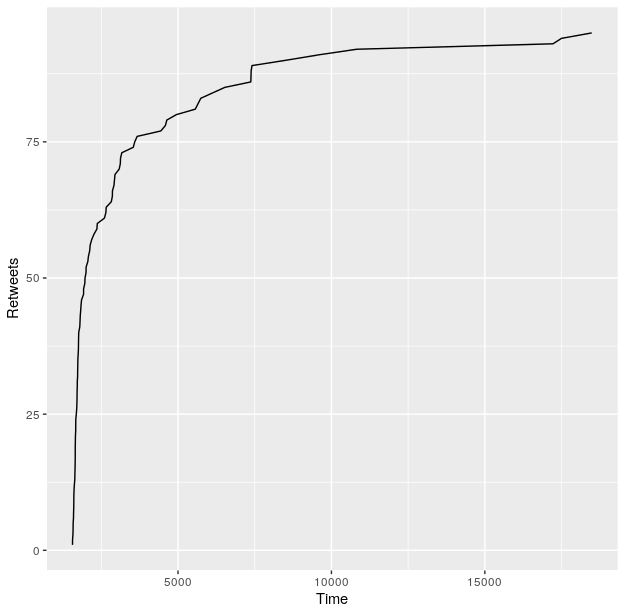
\includegraphics[width=.8\linewidth]{./Figures/maxRTcurve.png}
	  \caption{Maximum RT tweet distribution}
	  \label{fig:sub1}
	\end{subfigure}%
	\begin{subfigure}{.4\textwidth}
	  \centering
	  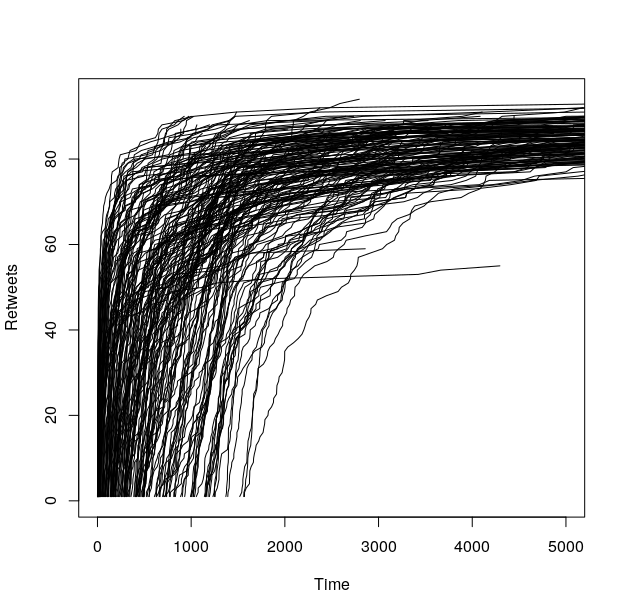
\includegraphics[width=1.05\linewidth]{./Figures/all_tweets.png}
	  \caption{All tweets distribution}
	  \label{fig:sub2}
	\end{subfigure}
\end{figure}

Each retweet counting process is defined by a time series, measuring the time for the next count (in minutes) since the creation of the tweet. 
That is, starting at $N_t=0, t=0$ the arrival times $s$ increases the count by 1 unit, fulfilling the condition $s<t, N_s \leq N_t$. Moreover, for any time $s<t$ the number of retweets in the interval $(s, t]$ is the difference $N_t -N_s$. 

Assuming that, if a user undoes a retweet, when acquiring the dataset the former time of retweet it is no longer recorded, the count can only increase and never decrease. 
The real model does not hold this assumption since this restriction is imposed by the internal functioning of Twitter and its API. 

i.e. The following sequence of times would define a retweet counting process for a tweet with 6 RT. 
Where the first event occurs after 1.4 minutes.

\begin{center}
\textit{1.400000    1.616667    1.716667    1.716667    1.900000    2.616667}
\end{center}

Knowing that, as stated in Section 6.7 of Dobrow RP \textit{Introduction to Stochastic Processes with R}, a nonhomogeneous Poisson process is a counting process $(N_t)_{t\geq0}$ with intensity function $\lambda(t)$ if
\begin{itemize}
	\item $N_0 = 0$ 
	\item For all $t>0$, $N_t$ has a Poisson distribution with mean
	\[\mathbb{E}[N_t] = \int^t_0\lambda(x)dx\]
	\item For $0\leq q < r \leq s < t$, $N_r - N_q$ and $N_t - N_s$ are independent random variables.
\end{itemize}

We know that the process already satisfies the conditions of a counting process. In order to find if it fits the hypothesis of a Poisson process, knowing that the times are not homogeneous, we will consider a non-homogeneous Poisson process.

When analysing time frequencies between times we notice that it decreases over time. Meaning that if it were to be a non-homogeneous Poisson process, for all $t>0$, $N_t$ it would follow a Poisson distribution with $\mathbb{E}[N_t] = \lambda = \int_{t}^{0} \lambda(x)dx$ where $\lambda_t < \lambda_{t+1}$ for all $t$ (difference greater over time), assuming unknown intensity function.

When plotting such distribution we get


\subsection{Assuming you can model the number of retweets by time as a non-homogeneous Poisson process with intensity function $ \lambda (t) = \theta e^{-\theta t},\ t>0$, graphically explore possible values of $\theta$ and choose the one that best fit your data. Explain all the considerations you make.}

In order to find the best $\theta$ possible, we need to simplify the problem. 
The first thing we perform is to find the mean poisson process of the Real Madrid twitter account. 
We can treat this mean poisson process as the expected retweet poisson process of a random tweet written in the Real Madrid account.

Because not all the tweets have the same amount of retweets we cannot calculate directly the mean value for a given time. 
In order to compute such value, first, all tweets times are interpolated to have the same amount of points (the number of points is equal to the number of retweets of the max RT tweet). 
Later, the values can simply be summed and divided by the total number of tweets. 
Once we have this mean line, we can plot it along with an arbitrary value of theta and compare visually.

\begin{figure}[H]
	\centering
	\begin{subfigure}{.4\textwidth}
	  \centering
	  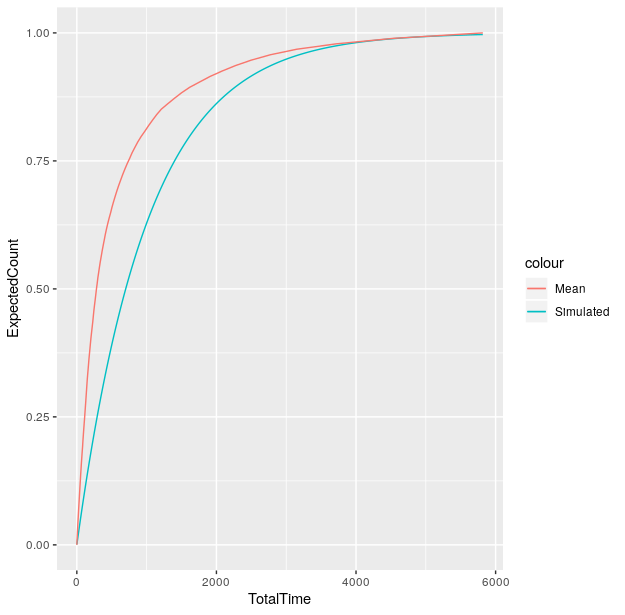
\includegraphics[width=0.9\linewidth]{./Figures/non_optimal.png}
	  \caption{Mean RT time of tweets and Simulated values with arbitrary $\theta$}
	  \label{fig:sub1}
	\end{subfigure}%
	\begin{subfigure}{.4\textwidth}
	  \centering
	  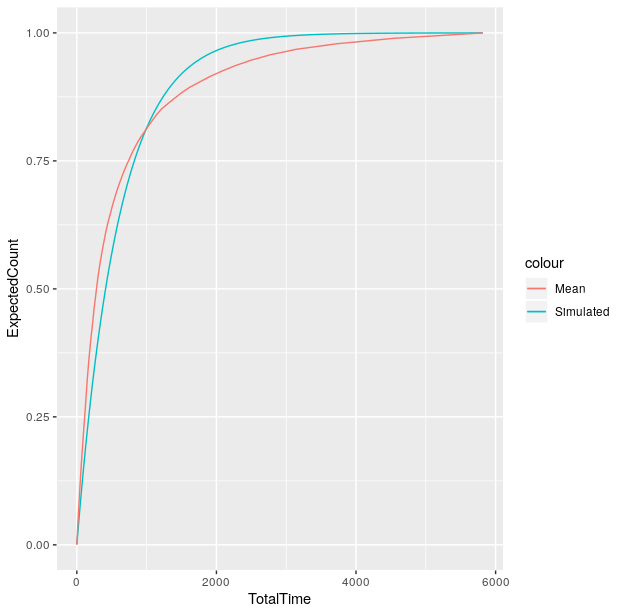
\includegraphics[width=1\linewidth]{./Figures/optimal.png}
	  \caption{Mean RT time of tweets and Simulated values with optimal $\theta$}
	  \label{fig:sub2}
	\end{subfigure}
\end{figure}

Once this two lines are plotted jointly, it is easily to see that an optimal value for $\theta$ would be the one that minimize the area between the two lines. 
That is exactly we did in the right plot. 
We write a function that automatically minimize this area and give us a value of $\theta=0.001683839$ with an area between lines of $173.1745$

\subsection{Write an R function to simulate data from a non-homogeneous Poisson process during a given time interval. Describe the inputs and outputs of your function.}

As stated in section 11.5.1 of Ross, Sheldon \textit{Introduction To Probability Models}, given $n$ events of a non-homogeneous Poisson process by time $T$ the $n$ event times are independent with a common density function
\[f(s) = \frac{\lambda(s)}{m(t)},\ 0<s<T, \quad m(T) = \int^T_0\lambda(s)ds\]

By simulating $N(T)$, the number of events by time T, and then simulating $N(T)$ random variables from the previous density function we can generate a NHPP.

\textbf{TODO Seguir explicando el algoritmo}

Translated into the following R function
\begin{lstlisting}[language=r]
simulateNHPP <- function(intensity_function, time, lambda_bound) {
	X <- numeric(0)
	
	for ( t in 1:time){
		u <- runif(2)
		accept <- u[2] <= intensity_function(time*u[1]) / lambda_bound
		if (accept)
			X <- c(X, time * u[1])
	}
		
	return(sort(X))
}
\end{lstlisting}
